\documentclass[a4paper, 12pt]{article}
\usepackage[utf8]{inputenc}
\usepackage{hyperref}
\usepackage{graphicx}
\graphicspath{ {./img/} }

\usepackage[italian]{babel}
%\usepackage[italian]{cleveref}

\title{\textbf{Relazione assignment 3}}
\author{Andrea Severi\\Daniel Rodilosso}
\date{a.a. 2021/2022}

\begin{document}

\maketitle

\section{Introduzione}
Si vuole realizzare un sistema IoT, implementando la simplificazione di un giardino smart, ovvero un sistema che controlla e monitora lo stato di un giardino. \'E formato da 5 componenti principali, elencate nella successiva sezione dedicata. Ulteriori informazioni si possono trovare al seguente \href{https://docs.google.com/document/d/1oD8VSHPsmvpfgtXeALszZn8Bt9sD60pmsZQmUkinLm0/edit}{\underline{\emph{link}}}\\
In alternativa, una dimostrazione visiva si trova al seguente \href{https://liveunibo-my.sharepoint.com/:v:/g/personal/andrea_severi12_studio_unibo_it/Ebr-YQ9bWPhForXCmn0dCDIBFiw2Ak20UQRDlxhNdCWyyQ?e=LvFZex}{\underline{\emph{link}}}

\section{Componenti}
\subsection{Garden Service}
Componente centrale del sistema in esecuzione sul PC. Utilizza Java e comunica direttamente con:
\begin{itemize}
    \item Sensoboard tramite protocollo HTTP per acquisizione dei dati riguardanti il
    giardino smart
    \item Dashboard tramite HTTP, postando i dati di cui necessita
    \item Controller tramite Seriale per inviare i dati che recupera dalla richiesta GET HTTP del Sensorboard
    \item App per l'invio dei dati tramite HTTP, come nel caso della Dashboard
\end{itemize}
\clearpage
\subsection{Garden Sensorboard}
Componente di acquisizione dei dati, si basa su ESP32. In particolare, recupera:
\begin{itemize}
    \item il valore della temperatura tramite il sensore LM35
    \item il valore della luminosità tramite la fotoresistenza LDR-VT90
\end{itemize}
Tali dati sono successivamente inviati tramite Wifi e protocollo HTTP al Service
\subsection{Garden Controller}
Costruito su Arduino Uno, tale componente agisce in base ai dati ricevuti tramite Seriale dal Service e tramite Bluetooth dall'App.\\
Sulla base dei valori recuperati, esegue determinate azioni quali:
\begin{itemize}
    \item accendere fino a 4 led
    \item azionare servo per l'irrigazione
\end{itemize}
\subsection{Garden Dashboard}
Componente interamente grafica che espone i dati ricevuti tramite richieste HTTP all'utente. Principalmente i dati ricevuti riguardano:
\begin{itemize}
    \item intensità della luminosità
    \item valore della temperatura
    \item stato attuale del giardino
\end{itemize}
\subsection{Garden App}
Si serve del Bluetooth per funzionare. Componente che comunica con Service e Controller. Dal primo ottiene i dati da esporre all'utente, al secondo trasmette le azioni che l'utilizzatore compie all'interno dell'applicazione. Alcune sono elencate di seguito:
\begin{itemize}
    \item cambiare lo stato del giardino
    \item accendere/spegnere fino a 4 led
    \item cambiare la velocità di irrigazione del servo all'interno del controller
    \item mettere in pausa l'irrigazione
\end{itemize}
\clearpage
\section{Schemi}
\begin{figure}[h]
    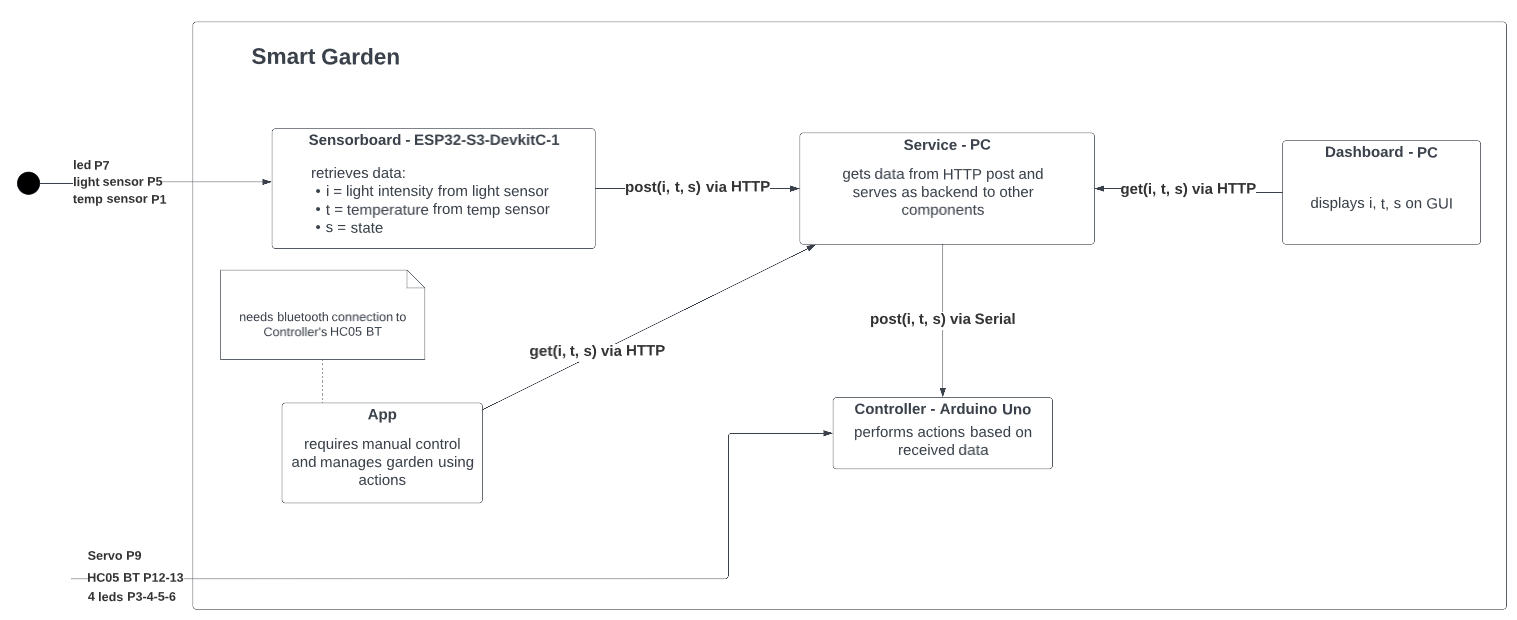
\includegraphics[scale=0.5]{general_smart_garden}
    \caption{Schema generale sul funzionamento del sistema}
\end{figure}

\begin{figure}[h]
    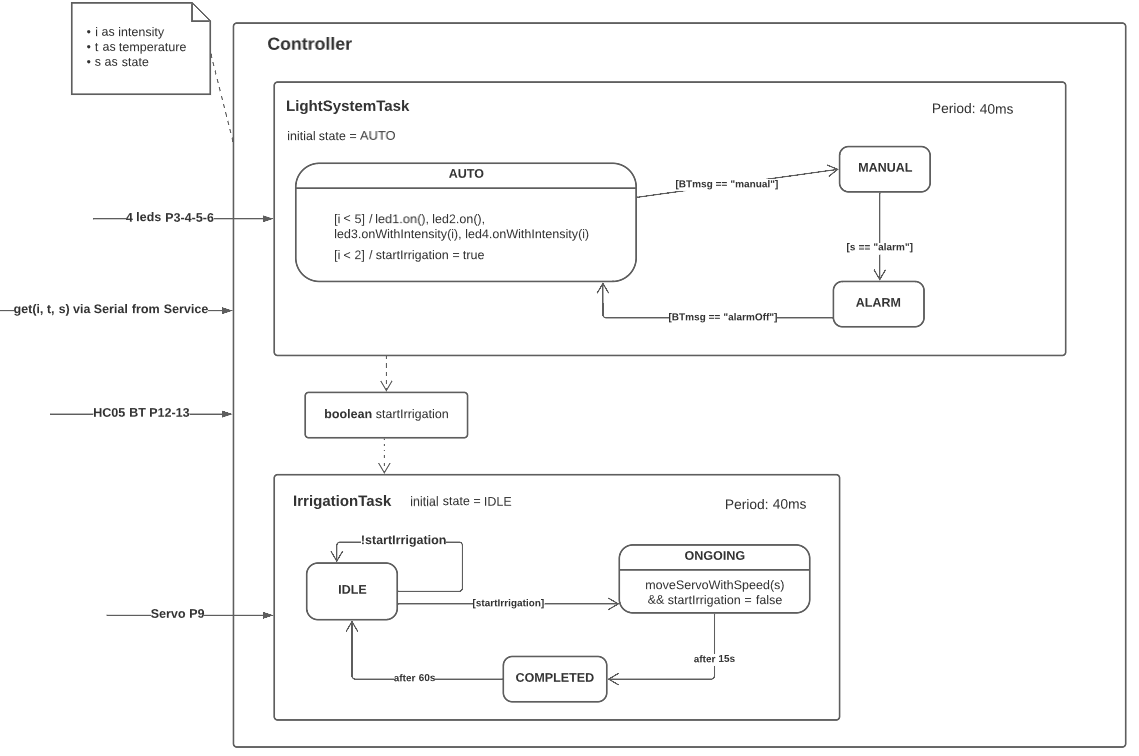
\includegraphics[scale=0.65]{controller_detail_smart_garden}
    \caption{Schema task controller}
\end{figure}

\begin{figure}[h]
    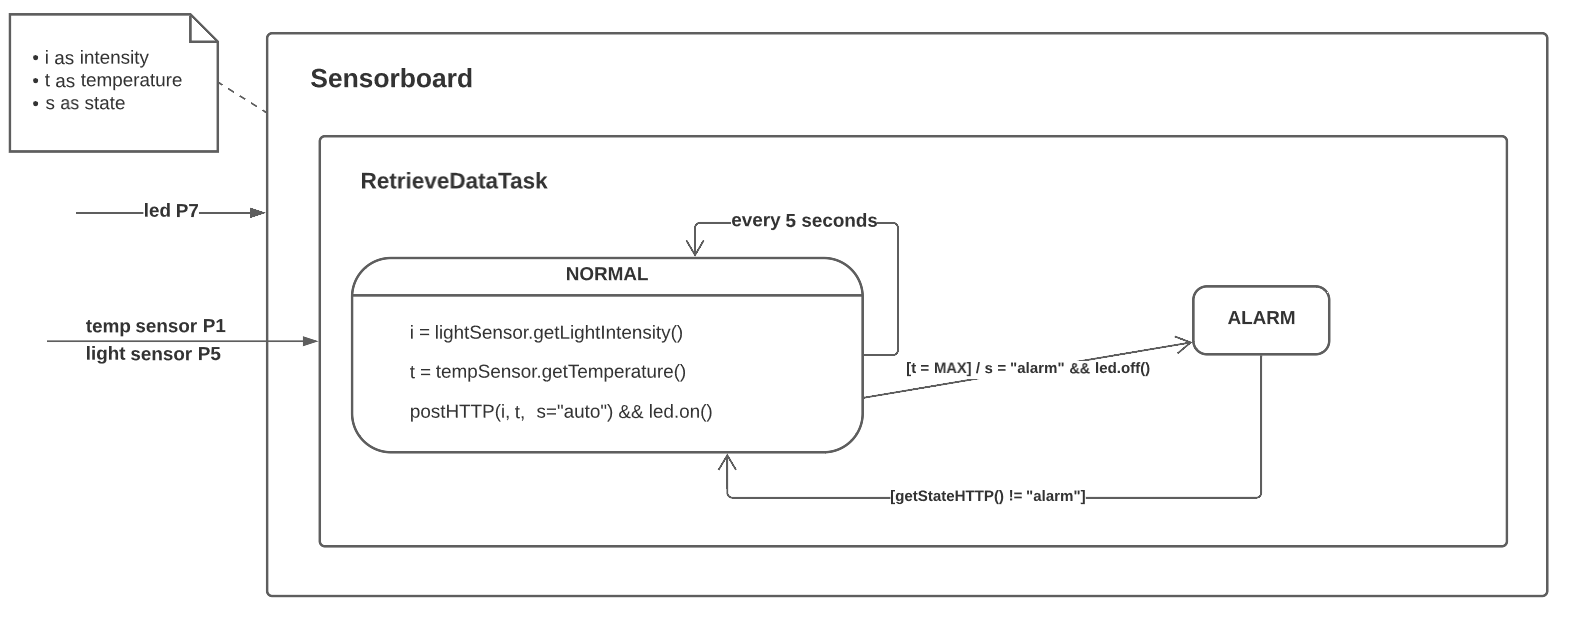
\includegraphics[scale=0.49]{sensorboard_detail_smart_garden}
    \caption{Schema task sensorboard}
\end{figure}



\end{document}
